\chapter{Conclusioni}
\label{cha:conclusioni}

Individuato il problema principale dell'implementazione precedente, con questi nuovi
sviluppi, il progetto SATAYO ha visto una rivisitazione completa del proprio
core. Per fare ciò sono state analizzate molte alternative all'architettura passata,
tra le quali alla fine è stata scelta la più adeguata secondo i requisiti
definiti durante la fase di analisi. Questo ha portato a un netto miglioramento della
capacità di analisi del sistema e ad una riduzione di risorse utilizzate in totale.

Durante l'analisi dell'applicazione e il processo di implementazione e migrazione
al nuovo sistema, sono state inoltre individuate altre aree in cui si potrebbero
apportare ulteriori migliorie. Sono riportate di seguito le principali e di più rilievo:

\begin{itemize}
  \item \textbf{Implementazione con Kubernetes:} è il prossimo sviluppo che
    emerge scontato dalla nuova implementazione. Come accennato al punto \ref{sec:impl_container}
    la configurazione dei container attuale, basata su Docker Compose, non è consigliata
    per carichi di lavoro di produzione. Per questo motivo è presente il \texttt{Helm
    Chart}\footnote{\url{https://helm.sh/docs/topics/charts/}} ufficiale messo a
    disposizione dagli sviluppatori di Airflow, il quale descrive l'infrastruttura
    ideale da dispiegare all'interno del cluster Kubernetes, per ottenere un
    funzionamento ottimale del sistema. Il Helm Chart permette inoltre di utilizzare
    immagini Docker personalizzate, permettendo quindi di usare direttamente l'immagine
    sviluppata per l'implementazione attuale. Questa miglioria, illustrata nell'immagine
    \ref{fig:infra_future}, porterà ad avere maggiore capacità di calcolo ed affidabilità
    all'interno di Airflow, permettendo quindi lo sviluppo riportato al prossimo
    punto;

  \item \textbf{Migrazione fasi Utility:} in ottica di manutenibilità del
    progetto e di standardizzazione dello stile del codice e delle regole di
    formattazione e linting, sarebbe opportuno migrare anche le fasi Utility al sistema
    Airflow. Dato il fatto che queste fasi hanno requisiti di isolamento
    particolari, per eseguire la migrazione è necessario testare a fondo il DockerOperator,
    introdotto nella sezione \ref{sec:airflow}, in modo tale da assicurarsi il corretto
    funzionamento delle fasi menzionate all'interno del nuovo ambiente;

  \item \textbf{Aggregazione e analisi dei log:} altra funzionalità, utile dal punto
    di vista del monitoraggio dell'esecuzione delle task, è sicuramente il
    collezionamento e l'aggregazione dei log. Sarebbe ideale utilizzare direttamente
    il servizio messo a disposizione da NetEye, che permetterebbe di indicizzare
    i messaggi di log completi prodotti dalle task di Airflow su Elasticsearch. In
    questo modo sarebbe possibile, oltre a consultare dettagliatamente i
    messaggi di log prodotti, creare una dashboard su Kibana\footnote{\url{https://www.elastic.co/kibana}}.
    Tale dashboard permetterebbe di avere visibilità su determinate tipologie di
    errore non critico che altrimenti verrebbe ignorato, rendendo possibile l'individuazione
    di bug che potrebbero portare alla perdita di informazione;

  \item \textbf{Pipeline di CI/CD e test automatizzati:} attualmente, la procedura
    di aggiornamento della versione di SATAYO Airflow viene effettuata manualmente.
    Sulla macchina di produzione vengono svolte le seguenti azioni: viene aggiornato
    il codice presente in locale, eseguita la procedura di build dell'immagine
    Docker, e infine vengono avviati i nuovi container basati sulla nuova versione.
    Tutte queste procedure potrebbero essere automatizzate tramite una pipeline
    di Continuous Deployment, responsabile di costruire l'immagine del Container,
    scaricarla, ed avviarla automaticamente sull'istanza di produzione. Avere a
    disposizione l'immagine, permetterebbe anche l'esecuzione di test automatizzati
    in un ambiente analogo a quello effettivo, permettendo quindi di testare
    automaticamente l'intera applicazione;

  \item \textbf{Notifiche intelligenti:} ultima feature molto valida potrebbe
    essere un sistema di notifiche immediate in caso di errori. Nello specifico verrebbe
    utilizzato un servizio di messaggistica istantanea, e.g. Telegram, per
    permettere la ricezione di notifiche in ogni momento. Gli eventi notificabili
    tramite questo sistema sarebbero principalmente errori critici di fasi di sistema
    e, secondariamente, errori di esecuzione delle task di SATAYO. Quest'ultima
    categoria di notifiche potrebbe portare in certi casi a spam indesiderato, per
    questo sarebbe opportuno attendere che le fasi di SATAYO raggiungano un'affidabilità
    tale da non risultare in troppe notifiche o, alternativamente, bisognerebbe implementare
    un rate limit per limitare le notifiche inviate.
\end{itemize}

\begin{figure}[htbp]
  \centering
  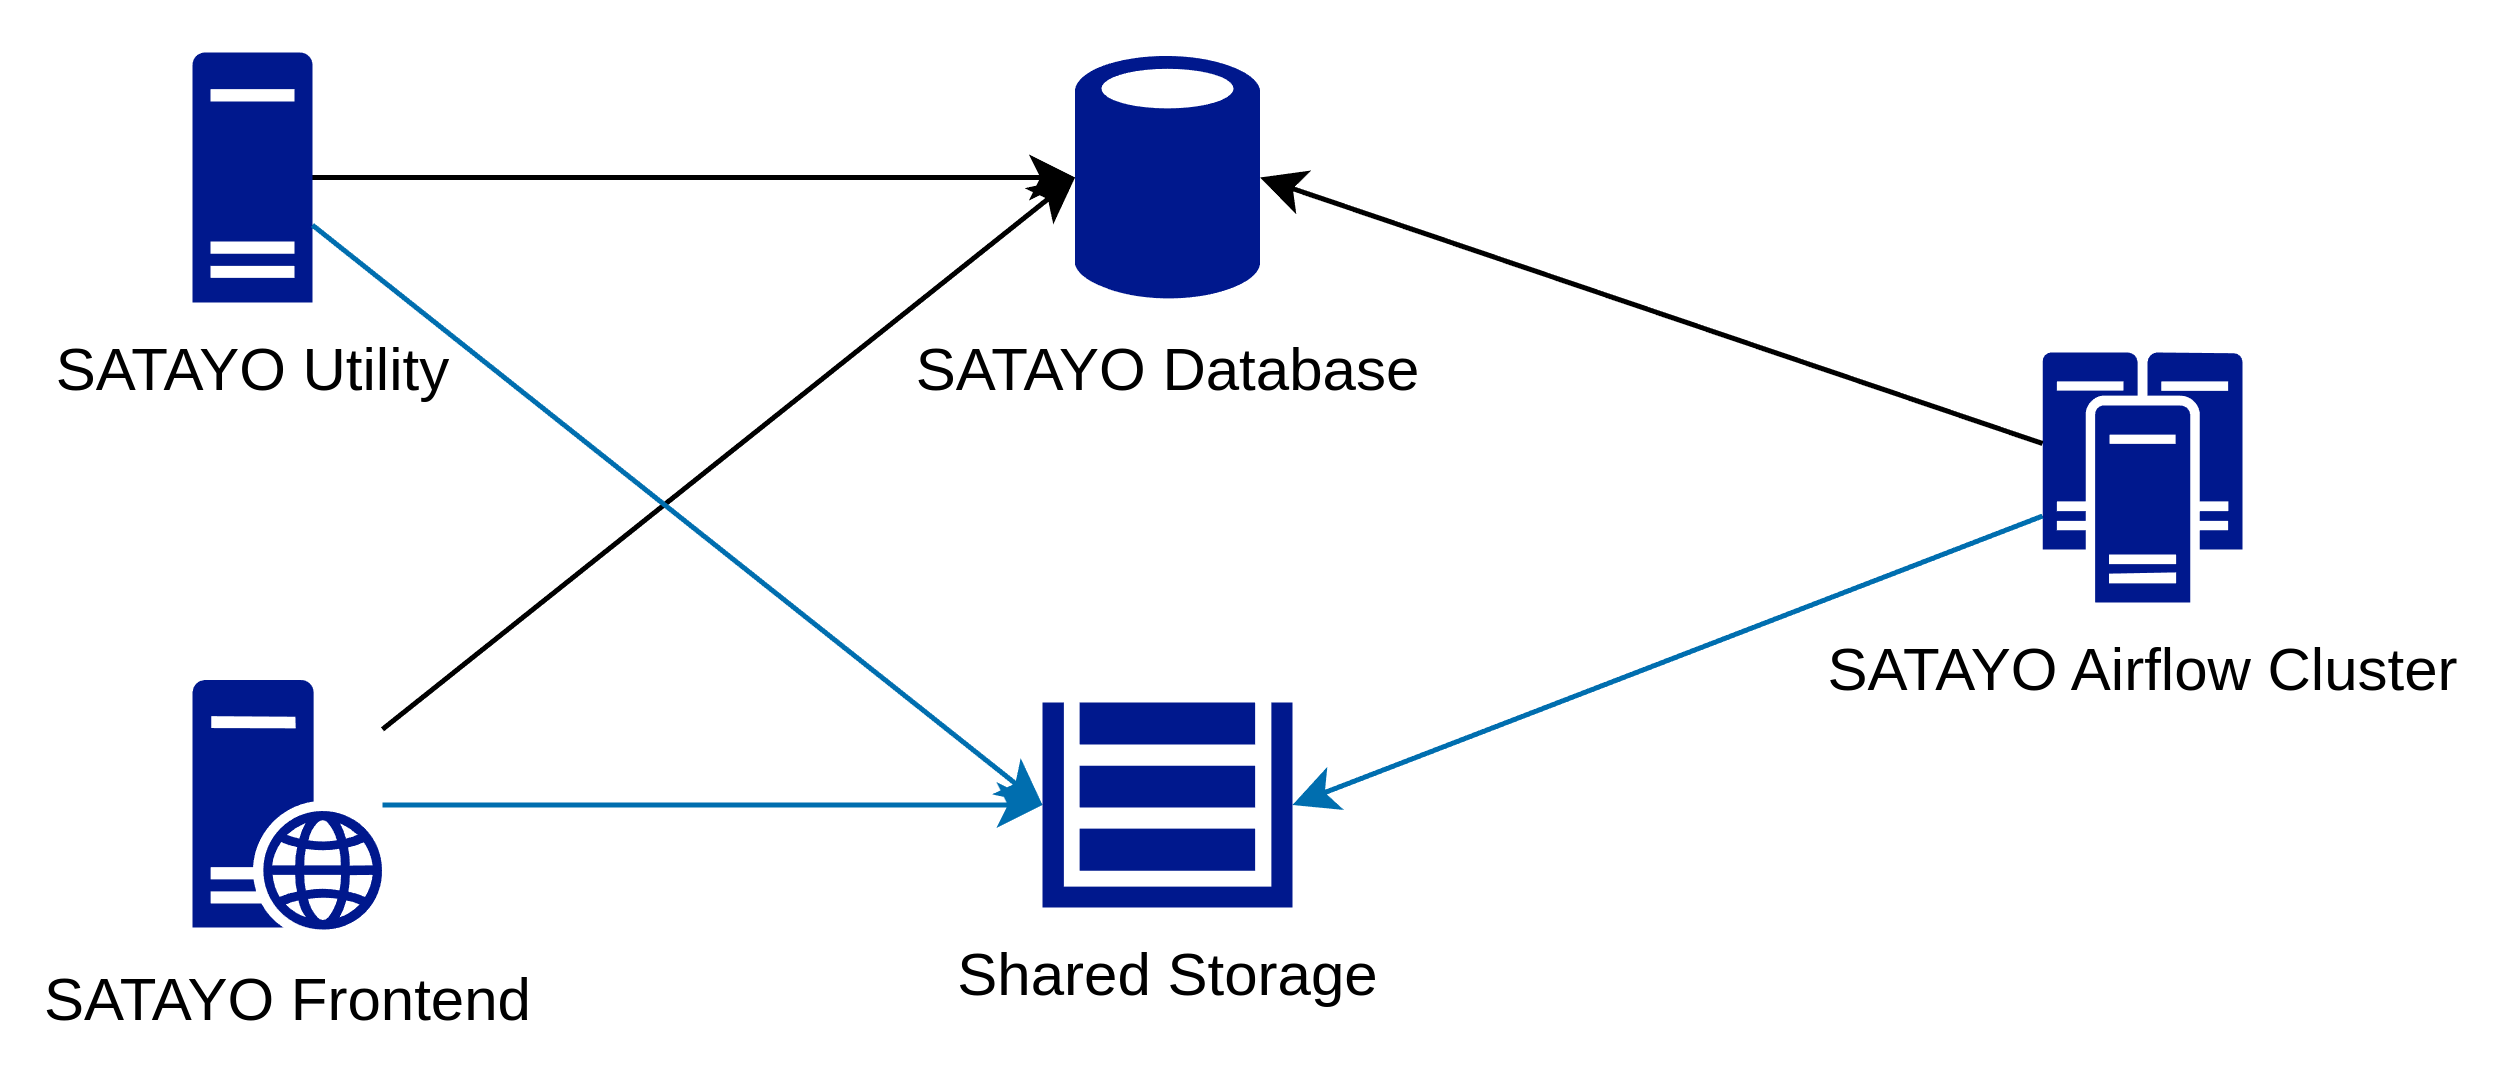
\includegraphics[width=.6\linewidth]{images/SATAYO_infrastructure_future.png}
  \caption{Futura infrastruttura di SATAYO}
  \label{fig:infra_future}
\end{figure}